\chapter{A New Theoretical Formalism}

In this chapter, a formalism that describes the wobbling properties in odd-$A$ nuclei will be presented. The model was developed recently by the current team (i.e., Raduta and Poenaru) and applied to $^{135}$Pr \cite{raduta2020new}, and the `Lu family' with $^{161,165,167}$Lu \cite{raduta2020approach} and $^{163}$Lu \cite{raduta2020approach,raduta2020towards,poenaru2021parity,poenaru2021extensive1,poenaru2021extensive2}. This framework is an original contribution to the field of nuclear structure, with focus on the theoretical aspects of collective phenomena in nuclei.

\section{Previous Work - Foundation}

From a development standpoint, it is instructive to review the previous `stages' that lead to the current work, since the description of odd-$A$ nuclei achieved in here is strongly connected with former calculations done by the team. Consequently, in this section a brief overview of the wobbling motion in $^{163}$Lu done by Raduta et al. in 2017 \cite{raduta2017semiclassical} will be given. Indeed, by using a \emph{semi-classical} approach, the wobbling properties of this odd-mass isotope were accurately described. 

The semi-classical approaches tend to be very useful when applied to problems having a \emph{quantal} Hamiltonian that contains quantities which behave as in the \emph{classical limit} when certain constraints or approximations are made. Moreover, these methods always keep the dynamics of the system in close contact with the classical features, which in principle are easier to interpret (i.e., a clear physical meaning). For this reason, the collective properties of $^{163}$Lu were characterized by such a method. Dealing with an odd nucleus it makes sense to adopt a Particle + Rotor Model in which the odd quasi-particle couples to an even-even core. From the total Hamiltonian $H=H_\text{rot}+H_\text{sp}$ (recall discussion on the PRM model \ref{triaxial-prm-general-hamiltonian} and also QTR Hamiltonian \ref{oddA-QTR-general-hamiltonian}), one obtained the energy spectrum for the four wobbling bands in this nucleus. Remarking the fact that there is another debate regarding the `true' nature of the fourth triaxial strongly-deformed band. For example, Jensen et al. \cite{jensen2004coexisting} suspect that this band is built from single-particle excitations, meaning that the states to not show wobbling mechanism. However, Tanabe et al. \cite{tanabe2008selection} is in favor of attributing $n_w=3$ for TSD4. More details on the interpretation of TSD4 will be discussed in the following sections.

After the initial Hamiltonian problem was established, classical equations of motions which fully describe the motion of $\mathcal{Q}$ and $\mathscr{C}$ (recall notations from Table \ref{notation-table-wobbling} that will still be used throughout the remaining chapters) are obtained through the Variational Principle (VP) by following a textbook procedure. The procedure of applying VP translates to the \emph{dequantization} procedure of an initial quantal Hamiltonian, thus making the change from a quantum space $S_\text{qt}$ to a classical space $S_\text{cls}$. This kind of transition $S_\text{qt}\to S_\text{cls}$ was also used previously for describing collective phenomena \cite{raduta2007semiclassical,chen2016two,budaca2018tilted}. For keeping a short overview of the foundational stage, the VP method applied to $H$ is skipped for now, but it will be detailed in a subsequent section. Furthermore, the classical equations of motions were solved with several restrictions, and the energy spectrum was analytically obtained (see Eq. 3.23 from the same reference). The excited bands TSD2, TSD3, and TSD4 were constructed via a phonon operator (denoted by $\Gamma_1^\dagger$ in Eq. 3.43 from \cite{raduta2017semiclassical}, which acts every state $I$). This approach makes it possible to have $n_w=3$ phonon excitations that are obtained by applying the phonon operator three times on the spin states belonging to the yrast band TSD1. In fact, since the states from TSD4 have negative parity, they are obtained by applying twice $\Gamma_1^\dagger(\pi=+1)$ and once $\Gamma_1^\dagger(\pi=-1)$, where the former phonon has positive parity and the latter has a negative parity. A schematic representation with the mechanism of action for the phonon operator from this formalism is shown in Fig. \ref{phonon-operator-schematic}.
\begin{figure}
    \centering
    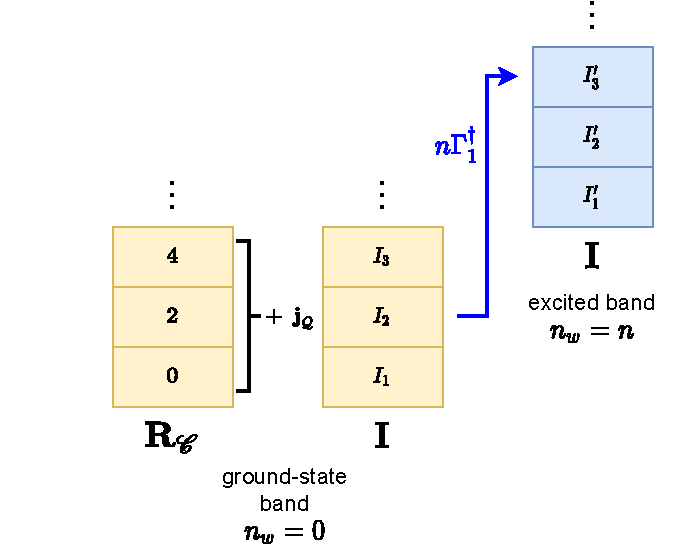
\includegraphics[width=0.75\textwidth]{Chapters/Figures/w0_phonon_operator.pdf}
    \caption{The mechanism of action for the phonon operator introduced in Ref. \cite{raduta2017semiclassical} for creating excited states of a given angular momentum, from the ground state bands. The core's angular momentum is defined as $\mathbf{R}_\mathscr{C}$, while the quasi-particle a.m. is denoted by $\mathbf{j}_\mathcal{Q}$. The ground-state band (yrast) emerges from the coupling of the quasi-particle with the triaxial core, giving rise to a series of spins $I_i=R_i+j$. By acting with $\Gamma_1^\dagger$ $n$-times on any of these states, then an excited level is obtained in a $n_w=n$ wobbling band. Keep in mind that one phonon operator increases the spin of a state by one unit.}
    \label{phonon-operator-schematic}
\end{figure}


From the seminal work from 2017 of the team, several features are emphasized:
\begin{itemize}
    \item The four TSD bands are considered as zero-, one-, two-, and three-wobbling phonon bands for TSD1, TSD2, TSD3, and TSD4, respectively
    \item Each excited band is obtained by acting on the yrast (TSD1) band with one-, two-, and three-phonons, respectively (e.g., a state $I$ from TSD2 is obtained by acting with the wobbling-phonon operator on a state $I-1$ from TSD1 and so on), according to Fig. \ref{phonon-operator-schematic}
    \item Wobbling structure for the group TSD1-2-3 emerged from a proton $i_{13/2}$ ($\mathcal{Q}_p$) where all spin states have positive parity
    \item The band TSD4 has spin states with negative parity, and it is built on a proton from the $h_{9/2}$ orbital (also a $\mathcal{Q}_p$)
    \item In the expression of the rotor Hamiltonian, the rigid-like MOI were adopted (see Eq. \ref{eq-irrotational-rigid-mois}) which depend on $\gamma$ and $\mathcal{I}_0$
    \item Analytical expressions for the energies were expressed in terms of total spin and wobbling phonon numbers
    \item Experimental data was reproduced through a fitting procedure, with the free parameters $\mathcal{I}_0^{-1}$ (rotor part) and a \emph{scaling factor} $s=V\cdot \mathcal{I}_0$ (single-particle part)
    \item The model assumes similar MOI across all four bands
    \item Deformation parameters $\beta_2$ and $\gamma$ were a priori fixed (taken from literature)
\end{itemize}

A year later, the team also extended this method into analyzing the wobbling properties of two more isotopes: $^{165,167}$Lu \cite{raduta2018wobbling}, and the model showed again that it was an useful tool in providing a realistic description of the wobbling motion in odd-mass nuclei. Hereafter, when referring to the procedure realized by Raduta and Poenaru in \cite{raduta2017semiclassical} and \cite{raduta2018wobbling}, the term $\mathbf{W_0}$ will be used. Throughout the following chapters, comparisons between the newly developed and improved theory and $\mathbf{W_0}$ will be made when necessary, in order to understand several key differences.

\section{Re-interpretation of The Wobbling Motion}

The $\mathbf{W_0}$ formalism can be regarded as a cornerstone in the description of an odd-$A$ particle-triaxial-rotor system done by the team. In a more recent follow-up work (2020) done by Raduta and Poenaru \cite{raduta2020approach,raduta2020towards}, a new interpretation of the wobbling bands was made, relative not only to the odd-$A$ $^{163}$Lu, but to an entire set of wobblers. The way of obtaining yrast and excited states within the collective spectrum turned out to be a first within literature, especially for $^{163}$Lu and $^{135}$Pr, since these nuclei have been drawing a lot of attention lately. The model starts with the typical QTR Hamiltonian:
\begin{align}
    \hat{H}=\hat{H}_\text{rot}+\hat{H}_\text{sp}\ ,
    \label{total-ham-approach-w1}
\end{align}
where $\hat{H}_\text{sp}$ represents the quasi-particle that moves inside the quadrupole mean-field as described in Eqs. \ref{eq-nilsson-ham-spherical-harmonics} and \ref{single-particle-nilsson-defored-potential} (recall discussion on the $\gamma$-deformed Nilsson potential and also Sections \ref{trm-model} - \ref{tprm-model}):
\begin{align}
    \hat{H}_\text{sp}=\epsilon_j+\frac{V}{j(j+1)}\left[\cos\gamma\left(3j_3^3-\mathbf{j}_\mathcal{Q}^2\right)-\sqrt{3}\sin\gamma\left(j_1^2-j_2^2\right)\right]\ ,
    \label{single-particle-ham-approach-w1}
\end{align}
with $\epsilon_j$ is the intrinsic energy of the particle from the corresponding $j$-shell (as it was discussed in Section \ref{tprm-model}). The total angular momentum of the odd-particle + core system is $\mathbf{I}=\mathbf{R}_\mathscr{C}+\mathbf{j}_{\mathcal{Q}_p}$. The components of the total angular momentum are: $$\mathbf{I}=\{\hat{I}_1,\hat{I}_2,\hat{I}_3\}\ ,$$ while the a.m. components for the $\mathcal{Q}_p$ are given as $$\mathbf{j}_{\mathcal{Q}_p}=\{\hat{j}_1,\hat{j}_2,\hat{j}_3\}\ .$$ The axes labelling for the triaxial ellipsoid is $(1,2,3)$. Knowing this, one can express the rotor part as:
\begin{align}
    \hat{H}_\text{rot}=\sum_{k=1}^3A_k(\hat{I}_k-\hat{j}_k)^2\ ,
    \label{rotor-ham-approach-w1}
\end{align}
where the inertial factors $A_k$ are expressed in terms of the three MOI:$$A_k=\frac{1}{2\mathcal{I}_k}\ .$$
Note that the Hamiltonian from Eq. \ref{rotor-ham-approach-w1} is just as the one expressed in Eq. \ref{general-rotor-hamiltonian}, except that here, the components of $\mathbf{R}_\mathscr{C}$ are given in terms of $\mathbf{I}$ and $\mathbf{j}_{\mathcal{Q}_p}$.

Obviously, the next task would be to obtained the eigenvalues of the Hamiltonian, which would comprise the energies of the system. One can proceed with the diagonalization procedure of $\hat{H}$ using a set of states that manifest the invariance to rotation by $\pi$ around a particular axis (the $D_2$ symmetry), since the Hamiltonian exhibits such a property. However, it is more practical to describe the system only though a few variables that have a classical counterpart. By doing this, the system dynamics will be close to the classical analogy of a rotating body lacking axial symmetry. The semi-classical approach that best fits this need os the Time-Dependent Variational Principle (TDVP), to which one associates the Time-Dependent Variational Equation (TDVE). When applying this Variational Principle on an initial problem, the requirement is to have a variational state which is constructed carefully, such that it embeds the necessary degrees of freedom of the underlying physics. Furthermore, VP will provide the time dependence of the variables that comprise the variational state itself \cite{budaca2018tilted}. Additionally, for each variable that parametrizes the state (usually the variables are complex), the TDVE will yield its equation of motion, thus finding the `connection' between the initial quantal variable (belonging to $S_\text{qt})$ and the classical variable (belonging to $S_\text{cls}$).

\subsection{Variational Principle}

The discussion regarding the TDVP and TDVE from above can therefore be summarized in the following equation, which must be associated to the quantum Hamiltonian ($\hat{H}\subset S_\text{qt}$) defined in Eq. \ref{total-ham-approach-w1}:
\begin{align}
    \delta\int_0^t\bra{\Psi_{IjM}}\hat{H}-i\frac{\partial}{\partial t'}\ket{\Psi_{IjM}}dt'=0\ .
    \label{tdve-approach-w1}
\end{align}
Obviously, the variational state $\ket{\Psi_{IjM}}\equiv\Psi_\text{trial}$ (also known as the \emph{trial function}) must be chosen in such a way that it comprises the entire space $S_\text{qt}$ of the original quantal Hamiltonian. This can be achieved if $\Psi_\text{trial}$ is a \emph{coherent state} \cite{glauber1963coherent}, which due to its \emph{completeness} property will span all the basis vector states from $S_\text{qt}$. Keep in mind that for $S_\text{qt}$ the states belong to the Hilbert space of $\hat{H}$. For the present case, the trial function is defined as:
\begin{align}
    \Psi_\text{trial}\equiv\ket{\Psi_{IjM}}=\mathcal{N}e^{z\hat{I}_-}e^{s\hat{j}_-}\ket{IMI}\ket{jj}\ ,
    \label{trial-function-appeoach-w1}
\end{align}
where the ladder operators for the total and single-particle a.m. are represented by $\hat{I}_-$ and $\hat{j}_-$, respectively. The factor $\mathcal{N}$ is the normalization constant, which keeps the trial function normalized to unity. Its value is given by \cite{raduta2007semiclassical,raduta2020new}:
\begin{align}
    \mathcal{N}=\left(1+|z|^2\right)^{-2I}\left(1+|s|^2\right)^{-2j}\ .
\end{align}
The states that are involved in $\Psi_\text{trial}$ are as follow: $\ket{IMK}$ represent the Wigner-D functions (i.e., eigenstates of $\hat{I}^2$ and $\hat{I}_3$), while $\ket{j\Omega}$ are the wave-functions of the odd quasi-particle $\mathcal{Q}$ (the eigenstates of $\hat{j}^2$ and $\hat{j}_-$). Notice that for both cases, the trial function contains their extremal form, namely the states of maximum projections $(K=I,\Omega=j)$. For $\ket{IMK}$, one has:
\begin{align}
    \ket{IMK}&=\sqrt{\frac{2I+1}{8\pi^2}}\mathcal{D}_{MK}^I\ , \nonumber\\
    \ket{IM-K}&=\sqrt{\frac{2I+1}{8\pi^2}}\mathcal{D}_{M-K}^I\ .
    \label{IMK-wigner-functions}
\end{align}
The second equation denotes the \emph{time-reversed} states, which are obtained by changing the projection $K$ to $-K$. The single-particle states can be defined more generally as:
\begin{align}
    \ket{\chi}&=\sum_{j\Omega}c_{j\Omega}\ket{\chi_{j\Omega}}=\sum_{j\Omega}c_{j\Omega}\ket{j\Omega}\nonumber\\
    \ket{\bar{\chi}}=&\sum_{j\Omega}c_{j-\Omega}\ket{\bar{\chi}_{j\Omega}}=\sum_{j\Omega}c_{j-\Omega}\ket{j-\Omega}=\sum_{j\Omega}(-1)^{j-1/2}c_{j\Omega}\ket{j-\Omega}\ .
    \label{j-Omega-single-particle-states}
\end{align}
The wave-functions are expressed in terms of the projections $\Omega=-j,\dots,j$. The states $\ket{\bar{\chi}_{j\Omega}}$ are the time-reversed ones and they are degenerate with $\ket{\chi_{j\Omega}}$. Because of the $D_2$ symmetry for $\hat{H}$, the total wave-function can be formulated as the a sum over the components $K, \Omega$ and over $j$. Denoting the total wave-function of the odd-mass nucleus as $\ket{\Psi}_\text{odd}$ (not to be confused with the trial function $\Psi_\text{trial}$), it must comprise both the intrinsic ($\mathbf{I}=\mathbf{R}_\mathscr{C}+\mathbf{j}_\mathcal{Q}$) and the single-particle ($\mathbf{j}_\mathcal{Q}$) degrees of freedom, namely:
\begin{align}
    \ket{\Psi_\text{odd}}&=\ket{\Psi_\text{intr.}}\otimes\ket{\Psi_\mathcal{Q}}=\nonumber\\
    &=\sqrt{\frac{2I+1}{16\pi^2}}\sum_K C_K\sum_{j,\Omega}c_{j\Omega}\left[\mathcal{D}_{MK}^I\ket{\chi_{j\Omega}}+(-1)^{I-j}\mathcal{D}_{M-K}^I\ket{\bar{\chi}_{j\Omega}}\right]=\nonumber\\
    &=\sqrt{\frac{2I+1}{16\pi^2}}\sum_K C_K \left[\mathcal{D}_{MK}^I\ket{\chi}+(-1)^{I-1/2}\mathcal{D}_{M-K}^I\ket{\bar{\chi}}\right]\ ,
    \label{total-wavefunction-oddA-general}
\end{align}
where the entire summation must be evaluated under the restriction $(K-\Omega)=even$. Such a restraint gives the allowed set of values for both $K$ and $\Omega$ to be:
\begin{align}
    \dots,-\frac{11}{2},-\frac{7}{2},-\frac{3}{2},\frac{1}{2},\frac{5}{2},\frac{9}{2},\frac{13}{2},\dots
\end{align}

Such states are from the quantal space $S_\text{qt}$, belonging to the Hamiltonian from Eq. \ref{total-ham-approach-w1}. Remarking the fact that for a known quasi-particle $\mathcal{Q}$ from a specific $j$-shell, one must keep $j$ constant within the summations. 

\subsection{Classical Equations of Motion}

Returning to the trial function $\ket{\Psi_{IjM}}$ from Eq. \ref{trial-function-appeoach-w1}, defined as a coherent state with products between  $\ket{IMK}$ (Eq. \ref{IMK-wigner-functions}) and $\ket{j\Omega}$ (Eq. \ref{j-Omega-single-particle-states}), its expression must be further discussed in terms of $z$ and $s$. Indeed, these two variables represent complex functions of time, and they are associated with the motion of the core and the odd-particle, respectively. Their expressions are:
\begin{align}
    z=\rho e^{i\varphi}\ ,\ s=\sigma e^{i\psi}\ .
\end{align}
The next step would be to evaluate the averages of both $\hat{H}$ and the time derivative $\frac{\partial}{\partial t}$ on the variational state $\ket{\Psi_{IjM}}$ as:
\begin{align}
    \left\langle \hat{H} \right\rangle&=\bra{\Psi_{IjM}}\hat{H}\ket{\Psi_{IjM}}\nonumber\\
    \left\langle \frac{\partial}{\partial t} \right\rangle&=\bra{\Psi_{IjM}}\frac{\partial}{\partial t}\ket{\Psi_{IjM}}\ .
    \label{hamiltonian-average}
\end{align}
The expressions of these quantities were defined in Ref. \cite{raduta2017semiclassical} with respect to the variables $z$ and $s$. However, it would be more useful to change the form of $\rho$ and $\sigma$ in the following way:
\begin{align}
    \rho \to r&=\frac{2I}{1+\rho^2}\ ,\ 0\leq r\leq 2I\ ,\nonumber\\
    \sigma \to f&=\frac{2j}{1+\sigma^2}\ ,\ 0\leq f\leq 2j\ .
    \label{changed-rho-sigma-variables}
\end{align}
These two new variables keep the same correspondence, meaning that $r$ is related to the core and $f$ is related to the odd-particle. Moreover, by doing such a transformation, the TDVE (Eq. \ref{tdve-approach-w1}) will provide the equations of motion in a canonical form (unlike the initial $\rho$ and $\sigma$). In fact, this was the reason behind the change of variable. The set of equations of motion are:
\begin{align}
    \frac{\partial \mathcal{H}}{\partial r}=\dot{\varphi}\ ,\ \frac{\partial \mathcal{H}}{\partial \varphi}=-\dot{r}\ ,\nonumber\\
    \frac{\partial \mathcal{H}}{\partial f}=\dot{\psi}\ ,\ \frac{\partial \mathcal{H}}{\partial \psi}=-\dot{f}\ ,
    \label{eq-of-motion-approach-w1}
\end{align}
where $\mathcal{H}$ is just the average of $\hat{H}$ on the trial function, as defined in Eq. \ref{hamiltonian-average}. It now plays the role of \emph{classical energy function} (CEF) and moreover, it is a constant of motion, implying that the energy of the system must be conserved. Remarking the fact that the \emph{classical image} of the initial problem (i.e., the Hamiltonian of an odd-$A$ triaxial nucleus) is now properly reached, through the equations of motion (Eq. \ref{eq-of-motion-approach-w1}) in the canonical form. The explicit form of the equations of motion provided by VP are:
\begin{align}
    \dot{\varphi}=&\frac{2i-1}{I}(I-r)\left(A_1\cos^2\varphi+A_2\sin^2\varphi-A_3\right)-\nonumber\\
                 &-2\sqrt{\frac{f(2j-f)}{r(2I-r)}}(I-r)\left(A_1\cos\varphi\cos\psi+A_2\sin\varphi\sin\psi\right)+2A_3(j-f)\ ,\nonumber\\
    \dot{\psi}=&\frac{2j-1}{j}(j-f)\left(A_1\cos^2\psi+A_2\sin^2\psi-A_3\right)-\nonumber\\
               &-2\sqrt{\frac{r(2I-r)}{f(2j-f)}}(j-f)\left(A_1\cos\varphi\cos\psi+A_2\sin\varphi\sin\psi\right)+2A_3(I-r)-\nonumber\\
               &-V\frac{2j-1}{j^2(j+1)}(j-f)\sqrt{3}\left(\sqrt{3}\cos\gamma+\sin\gamma\cos2\psi\right)\ , \nonumber\\
    \label{eq-of-motion-explicit-coordinates}
\end{align}
for the canonical coordinates $(\varphi,\psi)$, and:
\begin{align}
    -\dot{r}=&\frac{2I-1}{2I}r(2I-r)(A_2-A_1)\sin2\varphi+\nonumber\\
             &+2\sqrt{rf(2I-r)(2j-f)}\left(A_1\sin\varphi\cos\psi-A_2\cos\varphi\sin\psi\right)\ ,\nonumber\\
    -\dot{f}=&\frac{2j-1}{2j}f(2j-1)(A_2-A_1)\sin2\psi+\nonumber+\\
             &+2\sqrt{rf(2I-r)(2j-f)}\left(A_1\cos\varphi\sin\psi-A_2\sin\varphi\cos\psi\right)+\nonumber\\
             &+V\frac{2j-1}{j^2(j+1)}f(2j-f)\sqrt{3}\sin\gamma\sin2\psi\ ,
    \label{eq-of-motion-explicit-momenta}
\end{align}
for the canonical momenta $(r,f)$, respectively.

Additionally, the \emph{classical coordinates} encompassed in $S_\text{cls}$ are the generalized momentum and generalized coordinates, which here are represented by $(r,f)$ and $(\varphi,\psi)$, respectively. Keep in mind that the two sets of equations of motion and canonical coordinates correspond to the core and the single-particle. Thus, the dequantization procedure was properly described, obtaining the classical dynamics of the system. 

\subsection{Classical Energy Function (CEF)}

Regarding the structure of the CEF, its expression in terms of the canonical variables is given as:
\begin{align}
    \mathcal{H}&\equiv\bra{\Psi_{IjM}}\hat{H}\ket{\psi_{IjM}}=\nonumber\\
    &=\frac{I}{2}(A_1+A_2)+A_3I^2+\frac{2I-1}{2I}r(2I-r)\mathcal{A}_\varphi+\frac{j}{2}(A_1+A_2)+A_3j^2+\nonumber\\
    &+\frac{2j-1}{2j}f(2j-f)\mathcal{A}_\psi-2\sqrt{rf(2I-r)(2j-f)}\mathcal{A}_{\varphi\psi}+\nonumber\\
    &+A_3\left[r(2j-f)+f(2I-r)\right]-2A_3Ij+V\frac{2j-1}{j+1}\mathcal{A}_\gamma\ .
    \label{full-classical-energy-function}    
\end{align}
Since the expression is quite lengthy, some \emph{canonical factors} were introduced in Eq. \ref{full-classical-energy-function}, namely $\mathcal{A}_\varphi$, $\mathcal{A}_\psi$, $\mathcal{A}_{\varphi\psi}$, and $\mathcal{A}_\gamma$. They depend on the canonical coordinates as follows:
\begin{align}
    \mathcal{A}_\varphi&=A_1\cos^2\varphi+A_2\sin^2\varphi-A_3\ ,\nonumber\\
    \mathcal{A}_\psi&=A_1\cos^2\psi+A_2\sin^2\psi-A_3\ ,\nonumber\\
    \mathcal{A}_{\varphi\psi}&=A_1\cos\varphi\cos\psi+A_2\sin\varphi\sin\psi\ ,\nonumber\\
    \mathcal{A}_\gamma&=\cos\gamma-\frac{f(2j-f)}{2j^2}\sqrt{3}\left(\sqrt{3}\cos\gamma+\sin\gamma\cos2\psi\right)\ .
    \label{classical-energy-function-A-factors}
\end{align}

\subsubsection{Canonical Factors - Qualitative Analysis}

It is worth analyzing the behavior of the canonical factors defined in Eq. \ref{classical-energy-function-A-factors}, since their evolution with respect to the generalized coordinates and MOI ordering will provide a better understanding regarding the behavior of the CES, as it will be shown in the following sections. Firstly, the factor $\mathcal{A}_\varphi$ is graphically represented for different orderings of the inertia parameter $A_k$. This is shown in Fig. \ref{fig-A-varphi-canonical}. Because both $\mathcal{A}_\varphi$ and $\mathcal{A}_\psi$ have similar expressions (only the coordinate is changed), the plots are equivalent.
\begin{figure}
    \centering
    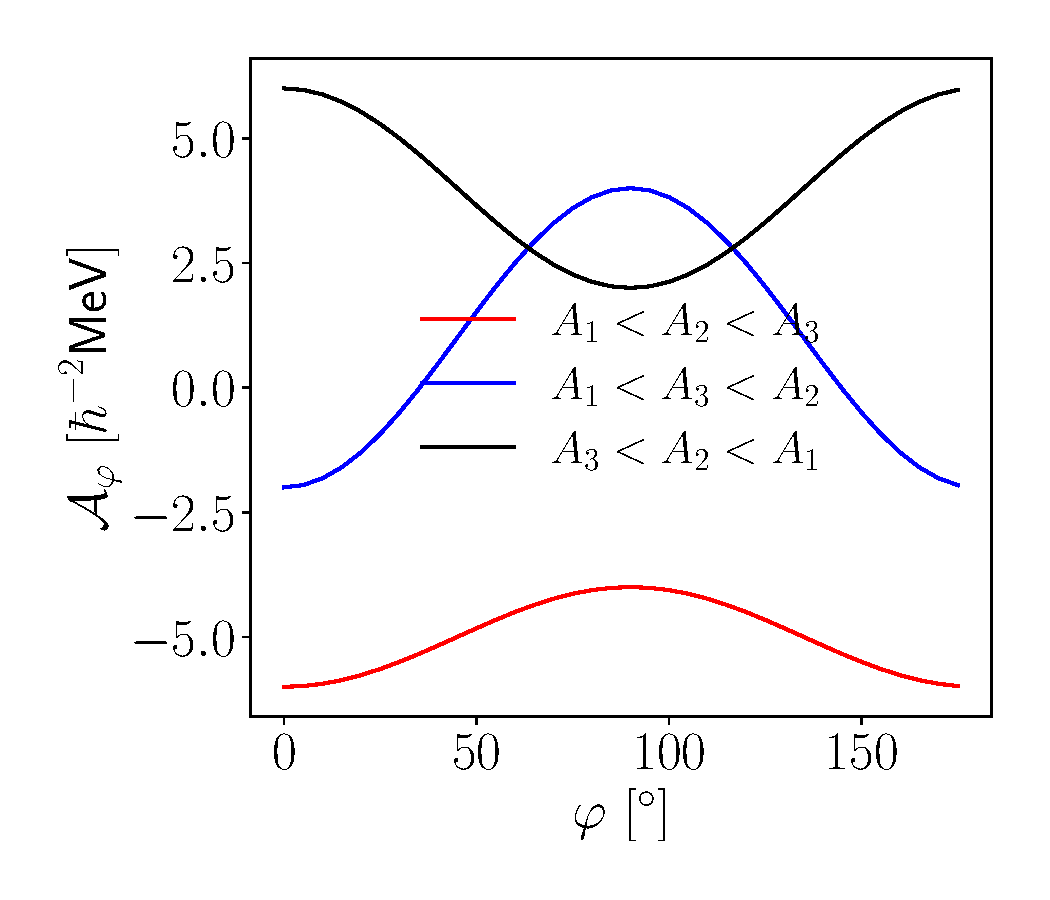
\includegraphics[width=0.49\textwidth]{Chapters/Figures/A_varphi_1.pdf}
    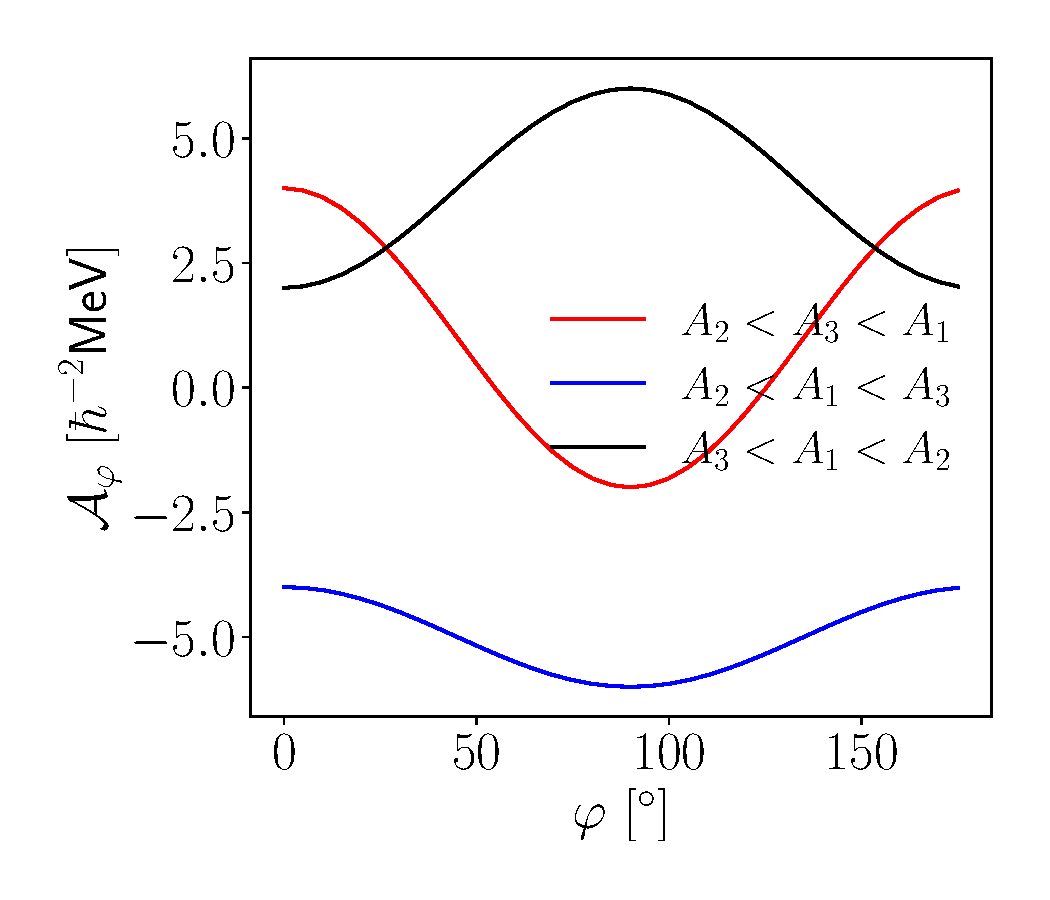
\includegraphics[width=0.49\textwidth]{Chapters/Figures/A_varphi_2.pdf}
    \caption{The evolution of $\mathcal{A}_\varphi$ with respect to the generalized coordinate $\varphi$, at different MOI orderings. The values $1,3,7$ were chosen and they are interchanged between the three inertia factors. This figure is equivalent for $\mathcal{A}_\psi$.}
    \label{fig-A-varphi-canonical}
\end{figure}

For the mixed term $\mathcal{A}_{\varphi,psi}$ from Eq. \ref{classical-energy-function-A-factors} it is more suitable to create a contour plot, since it depends on both canonical coordinates $(\varphi,\psi)$. As such, representations with different MOI orderings have been depicted in Fig. \ref{fig-A-mixed-canonical}, by lettings both coordinates vary inside the interval $[0,\pi]$.
\begin{figure}
    \centering
    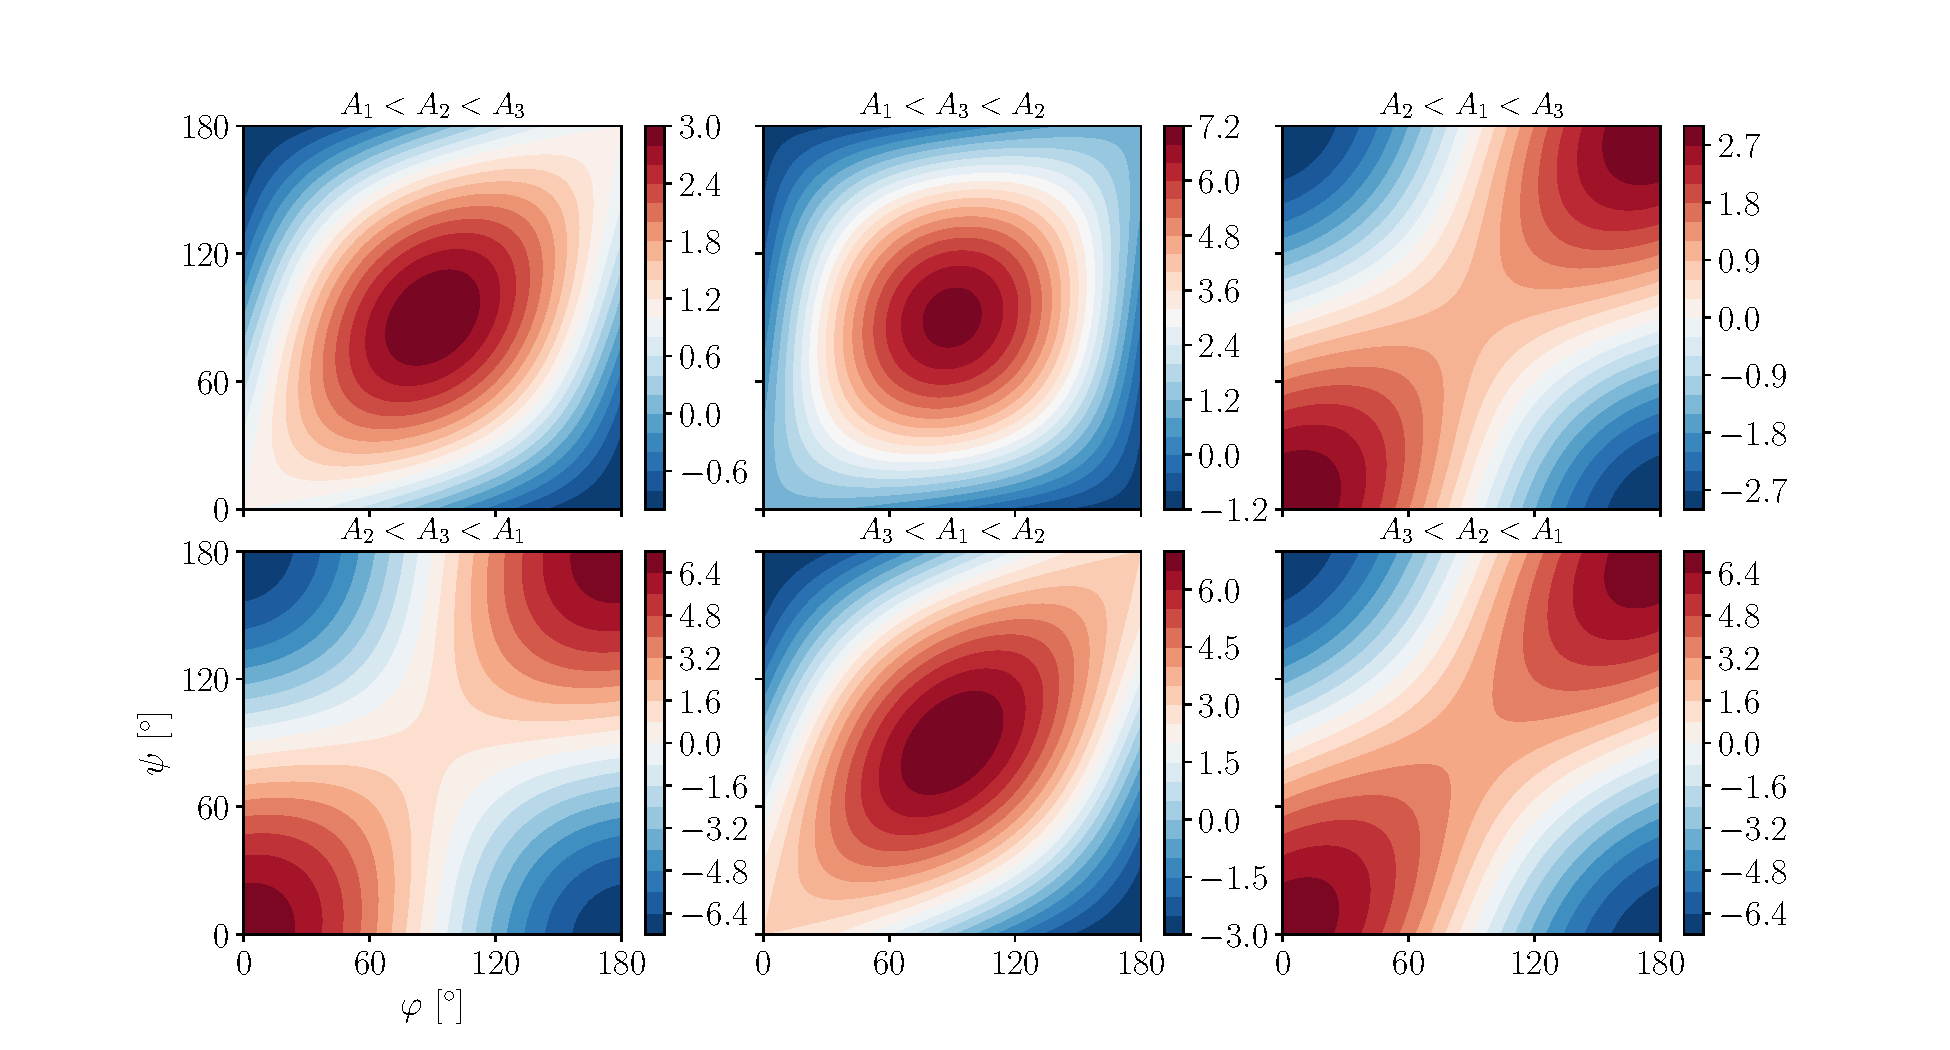
\includegraphics[width=0.99\textwidth]{Chapters/Figures/A_mixed.pdf}
    \caption{The mixed canonical factor $\mathcal{A}_{\varphi\psi}$ from Eq. \ref{classical-energy-function-A-factors}, as function of the coordinates $\varphi$ and $\psi$. Both variables vary within the interval $[0,\pi]$. All insets share a common labelling for the OX and OY axes.}
    \label{fig-A-mixed-canonical}
\end{figure}

Lastly, the factor $\mathcal{A}_gamma$ must also be represented as a contour plot, because it depends on the canonical coordinates of the single-particle, namely the set $(f,\psi)$. Its graphical representation for a few values of $\gamma$ shown in Fig. \ref{fig-A-gamma-canonical}.
\begin{figure}
    \centering
    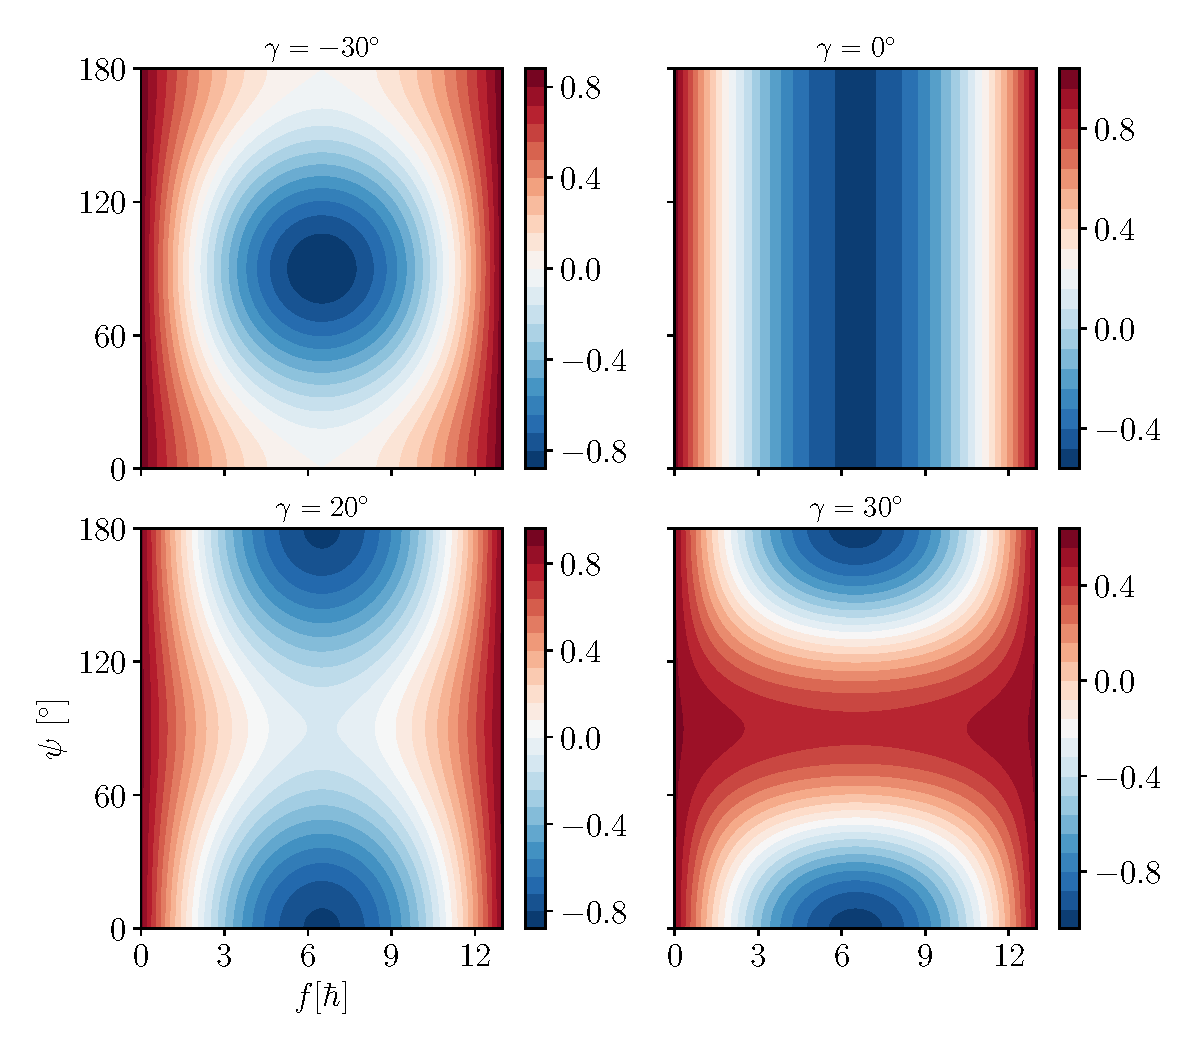
\includegraphics[width=0.99\textwidth]{Chapters/Figures/A_gamma.pdf}
    \caption{The canonical factor $\mathcal{A}_\gamma$ from Eq. \ref{classical-energy-function-A-factors}, as a function of the coordinates $(f,\psi)$ corresponding to the single-particle $\mathcal{Q}$. The $j$-shell has been fixed to $j=13/2$. In terms of the two variables, $f$ varies within $[0,2j]$ while $\psi$ is inside the interval $[0,\pi]$. All insets share a common labelling for the OX and OY axes.}
    \label{fig-A-gamma-canonical}
\end{figure}

From the representations shown in Figs. \ref{fig-A-varphi-canonical} - \ref{fig-A-gamma-canonical}, one can interpret the results as possible conditions for stability of an odd-$A$ system with regards to the triaxial wobbling regime. More precisely, the smaller the values of $\mathcal{A}$ are, a higher tendency for the system to achieve a lower total energy will arise. Keep in mind that all these canonical factors take part in the structure of the CEF. Consequently, lower energy could imply a greater level of stability.

\subsubsection{Critical Region}

Given the general expression of the CEF from Eqs. \ref{full-classical-energy-function} - \ref{classical-energy-function-A-factors}, one can group the terms in a part that is independent on the coordinates, a part that depends only on the core's coordinates $(r,\varphi)$, a third part that depends on the single-particle's coordinates $(f,\psi)$, and finally a \emph{mixed} term, which contains both sets of classical coordinates. As a result, $\mathcal{H}$ can be summarized:
\begin{align}
    \mathcal{H}(r,\varphi;f,\psi)=\mathcal{H}_\text{free}+\mathcal{H}_\mathscr{C}(r,\varphi)+\mathcal{H}_\mathcal{Q}(f,\psi)+\mathcal{H}_\text{mixed}(r,\varphi;f,\psi)\ .
    \label{classical-energy-function-terms}
\end{align}
From the critical conditions associated to the classical energy function, namely:
\begin{gather*}
    \left(\frac{\partial \mathcal{H}}{\partial r}\right)=0\ ,\ \left(\frac{\partial \mathcal{H}}{\partial \varphi}\right)=0\ ,\\
    \left(\frac{\partial \mathcal{H}}{\partial f}\right)=0\ ,\ \left(\frac{\partial \mathcal{H}}{\partial \psi}\right)=0\ ,
\end{gather*}
it is possible to obtain the points at which $\mathcal{H}$ is \emph{minimal} (provided by the sign of its corresponding Hessian). In order to meet such a criteria for $\mathcal{H}$, one needs to set an ordering of the three inertia factors. Choosing the largest MOI to be around the $3$-axis and $\mathcal{I}_3>\mathcal{I}_2>\mathcal{I}_1$ (or, equivalently $A_1<A_2<A_3$), the function achieves a minimum value at $p_0=(I,0;j,0)$.

\subsection{Wobbling Frequencies}

By performing a linearization procedure on the classical equations of motion (from Eq. \ref{eq-of-motion-approach-w1} or explicitly in Eqs. \ref{eq-of-motion-explicit-coordinates} - \ref{eq-of-motion-explicit-momenta}) around the minimum point of $\mathcal{H}$ (i.e., point $p_0$), an algebraic equation of fourth degree will show up, with a new variable which will be denoted with $\Omega$. Reasoning behind this labelling will become clear later on. For now, the equation for $\Omega$ is given generally as:
\begin{align}
    \Omega^4+B\Omega^2+C=0\ ,
    \label{omega-equation-linearized}
\end{align}
where the coefficient $B$ is:
\begin{multline}
    B=-\bigg\{\left[ (2I-1)(A_3-A_1)+2jA_1\right]\left[(2I-1)(A_2-A_1)+2jA_1\right]+8A_2A_3Ij+\\
    +\left[(2j-1)(A_3-A_1)+2IA_1+V\frac{2j-1}{j(j+1)}\sqrt{3}\left(\sqrt{3}\cos\gamma+\sin\gamma\right)\right]\cdot\\
    \left.\cdot\left[(2j-1)(A_2-A_1)+2IA_1+V\frac{2j-1}{j(j+1)}2\sqrt{3}\sin\gamma\right]\right\}\ ,
    \label{omega-B-term}
\end{multline}
and the coefficient $C$ is:
\begin{multline}
    C=\bigg\{\left[(2I-1)(A_3-A_1)+2jA_1\right]\bigg[(2j-1)(A_3-A_1)+2IA_1+\\
    +V\frac{2j-1}{j(j+1)}\sqrt{3}(\sqrt{3}\cos\gamma+\sin\gamma)\bigg]-4IjA_3^2\bigg\}\bigg\{\left[(2I-1)(A_2-A_1)+2jA_1\right]\cdot\\
    \cdot\left[(2j-1)(A_2-A_1)+2IA_1+V\frac{2j-1}{j(j+1)}2\sqrt{3}\sin\gamma\right]-4IjA_2^2\bigg\}\ .
    \label{omega-C-term}
\end{multline}
In a work done by Raduta et al \cite{raduta2017semiclassical}, a similar equation as the one from Eq. \ref{omega-equation-linearized} was obtained via a Random Phase Approximation (RPA) method applied to another (quantized) energy function. It is of crucial importance to extract from Eq. \ref{omega-equation-linearized} only those solutions that are real and positive, so one has to study the stability conditions for the equation. Deriving certain restriction on the parameters involved in $B$ and $C$ is therefore required. Obviously, the solutions to the general equation are:
\begin{align}
    \Omega_1 \to \left(\frac{-B-\sqrt{B^2-4 C}}{2}\right)^{1/2}\ ,&\ \Omega_2 \to \left(\frac{-B+\sqrt{B^2-4 C}}{2}\right)^{1/2}\ ,\nonumber\\
    \Omega_3 \to -\left(\frac{-B-\sqrt{B^2-4 C}}{2}\right)^{1/2}\ ,&\ \Omega_4 \to -\left(\frac{-B+\sqrt{B^2-4 C}}{2}\right)^{1/2}\ .
    \label{omega-1-2-3-4-solutions}
\end{align}
Since the positiveness condition mentioned above, it is clear that only $\Omega_1$ and $\Omega_2$ will be taken into consideration. The conditions where Eq. \ref{omega-equation-linearized} has vanishing solutions will be now analyzed in terms of $B$ and $C$.

\textit{Case i)} $B>0$ \textit{and} $C=0$

The situation $C=0$ imposes that the terms (or at least one) inside the curly brackets from Eq. \ref{omega-C-term} will equate to zero. In order to simplify the calculations, some notations should be introduced. Firstly, from the definition of $A_k=1/(2\mathcal{I}_k)$ one can exploit the fact that MOI (both in rigid representation as well as the irrotational ones) are typically expressed in terms of $\beta_2$, $\gamma$, and a common term (recall Eq. \ref{eq-irrotational-rigid-mois}):
\begin{align}
    \mathcal{I}_k=\mathcal{I}_0\cdot h(\beta_2,\gamma;k)\ ,
\end{align}
where $h$ is a trigonometric function defining moments of inertia either in the rigid picture or in the irrotational picture. Going back to the inertia factors, it results that:
\begin{align}
    A_k=\frac{1}{2\mathcal{I}_k}=\frac{1}{\mathcal{I}_0}\cdot h'(\beta_2,\gamma;k)\equiv\frac{1}{\mathcal{I}_0}\bar{A}_k\ .
    \label{A-bar-general}
\end{align}
Using thus Eq. \ref{A-bar-general}, each sub-term from $B$ and $C$ can be re-written with the following notations:
\begin{align}
    P_{31}&=(2I-1)(\bar{A}_3-\bar{A}_1)+2j\bar{A}_1\ ,\ P_{21}=(2I-1)(\bar{A}_2-\bar{A}_1)+2j\bar{A}_1\ , \nonumber\\
    Q_{31}&=(2j-1)(\bar{A}_3-\bar{A}_1)+2I\bar{A}_1\ ,\ Q_{21}=(2j-1)(\bar{A}_2-\bar{A}_1)+2I\bar{A}_1\ ,\nonumber\\
    G_1&=\frac{2j-1}{j(j+1)}\sqrt{3}\left(\sqrt{3}\cos\gamma+\sin\gamma\right)\ ,\ G_2=\frac{2j-1}{j(j+1)}2\sqrt{3}\sin\gamma\ .
\end{align}
This transformation is very useful because the constant $1/\mathcal{I}_0$ can be factored out from both $B$ and $C$, leaving only one `independent variable' within equations, namely $S=\mathcal{I}_0V$, which will be considered a \emph{scaling factor}. Getting back to $C=0$, after some rearrangement one gets:
\begin{align}
    P_{31}G_1S+P_{31}Q_{31}-4Ij\bar{A}_3^2=&0\ ,\nonumber\\
    P_{21}G_2S+P_{21}Q_{21}-4Ij\bar{A}_2^2=&0\ .
    \label{S-parameter-equations-set1}
\end{align}
Indeed, the above formulas represent a set of linear equations in the newly introduced variable $S$, which are of the form $aS+b=0$. As a physical interpretation for $S$, it is remarkable the fact that it comprises both a rotational part of the odd-mass system (through $\mathcal{I}_0$) but also single-particle contribution (through the potential strength $V$) so it \emph{encodes} the effect of collective rotation and deformation. By a straightforward manipulation of Eq. \ref{S-parameter-equations-set1}, the two solutions which provide vanishing a $C$ term are:
\begin{align}
    S_{01}=\frac{4Ij\bar{A}_3^2-P_{31}Q_{31}}{P_{31}G_1}\ \text{and}\ S_{02}=\frac{4Ij\bar{A}_2^2-P_{21}Q_{21}}{P_{21}G_2}\ .
    \label{C-Term-zero-solutions}
\end{align}

\textit{Case ii)} $B=0$ \textit{and} $C=\text{arbitrary}$

When $B$ must vanish, a second-degree algebraic equation for the variable $S$ will emerge. Using the same notations that where introduced in the case $i)$ for the sub-terms within $C$, it results:
\begin{align}
    P_{31}P_{21}+8Ij\bar{A}_2\bar{A}_3+\left(Q_{31}+SG_1\right)\left(Q_{21}+SG_2\right)=0\ , \nonumber
\end{align}
or:
\begin{align}
    G_1G_2S^2+\left(Q_{21}G_1+Q_{31}G_2\right)S+P_{31}P_{21}+8Ij\bar{A}_2\bar{A}_3=0\ .
    \label{S-parameter-equations-set2}
\end{align}
The solutions from this second-degree equation are:
\begin{align}
    S_{11}&=-\frac{\sqrt{\left(G_1 Q_{21}+G_2 Q_{31}\right){}^2-4 G_1 G_2 \left(8 I j \bar{A}_2 \bar{A}_3+P_{21} P_{31}\right)}+G_1 Q_{21}+G_2 Q_{31}}{2 G_1 G_2}\ ,\nonumber\\
    S_{12}&=\frac{\sqrt{\left(G_1 Q_{21}+G_2 Q_{31}\right){}^2-4 G_1 G_2 \left(8 I j \bar{A}_2 \bar{A}_3+P_{21} P_{31}\right)}-G_1 Q_{21}-G_2 Q_{31}}{2 G_1 G_2}\ .
    \label{B-Term-zero-solutions}
\end{align}
Gathering the outcomes from Eqs. \ref{B-Term-zero-solutions} and \ref{C-Term-zero-solutions}, four solutions for the variable $S$ were obtained, i.e., $S=\{S_{01},S_{02},S_{11},S_{12}\}$. 

Returning to the case $i)$ which provides vanishing $C$ term, it would be instructive to see for what values of $\mathcal{I}_0$ and $V$ the left-hand sides from Eq. \ref{S-parameter-equations-set1} equate to zero. Denoting the first left-hand side with $f_1=f_1(\mathcal{I}_0,V)$ and the second one with $f_2=f_2(\mathcal{I}_0,V)$, the contour lines that make $f_1$ and $f_2$ cancel out are represented in Fig. \ref{fig-vanishing-f1-f2}.
\begin{figure}
    \centering
    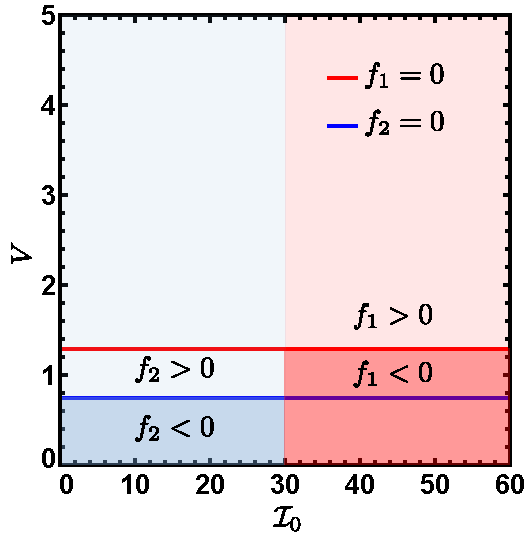
\includegraphics[scale=0.8]{Chapters/Figures/f1f2_solutions-edited.pdf}
    \caption{The contour lines show for which values of $\mathcal{I}_0$ and $V$ the left-hand sides from Eq. \ref{S-parameter-equations-set1} are zero. The two sides are denoted by $f_1$ and $f_2$, respectively. The calculations were done for fixed values of $I, j, \gamma, A_1, A_2, A_3$. Regarding the coloring, darker red corresponds to negative values of $f_1$, while lighter red means positive $f_1$. Similarly for the $f_2$ term with blue color. A 50/50 ratio for each color has been chosen relative to the width of the plot just for a clear difference between the positive/negative zones for the two functions.}
    \label{fig-vanishing-f1-f2}
\end{figure}

Furthermore, the left-hand side of Eq. \ref{S-parameter-equations-set2} from case $ii)$ can also be zero for certain intervals of $\mathcal{I}_0$ and $V$. A restriction on $V$ to only have positive values is adopted throughout the formalism (to be consistent with the literature \cite{shou2009coupling,tanabe2017stability,poenaru2021parity}). This forces only a single contour (denoted with $F=0$) to appear above the OX axis. A representation showing this line is done in Fig. \ref{fig-vanishing-F}, evaluated at arbitrary $I, j, \gamma, A_1, A_2, A_3$. Keep in mind that the $V$ parameter is restricted to the interval $[0,5]$ as it was the case for Fig. \ref{fig-vanishing-f1-f2}.
\begin{figure}
    \centering
    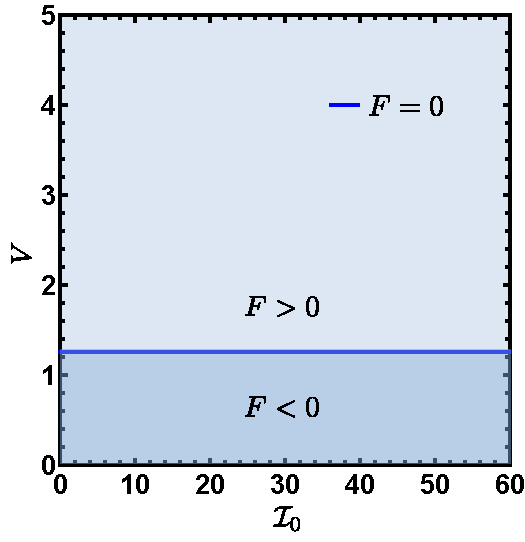
\includegraphics[scale=0.8]{Chapters/Figures/F_solutions_B-term.pdf}
    \caption{Graphical representation with the contour $F=0$ as function of the parameters $\mathcal{I}_0$ and $V$, where $F$ represents the left-hand side of Eq. \ref{S-parameter-equations-set2}. Arbitrary values for $I, j, \gamma, A_1, A_2, A_3$ were chosen. Darker color signifies negative values for $F$, while opposite holds for the lighter shading.}
    \label{fig-vanishing-F}
\end{figure}

Taking a look at the regions depicted in Figs. \ref{fig-vanishing-f1-f2} - \ref{fig-vanishing-F}, one can assume that they represent a clear indicator regarding the stability of Eq. \ref{omega-equation-linearized}. Obviously, when values of $(\mathcal{I}_0,V)$ lie near the contours lines within the plots, the equation reaches instability and no real solutions emerge.

Regarding the solutions given in Eq. \ref{omega-1-2-3-4-solutions}, the selected ones where $\Omega_1$ and $\Omega_2$. Considering their structure, it is important to retrieve all the conditions that grant positive square roots.